\documentclass[a4paper,10pt]{article}
\usepackage{titling}
\usepackage{fullpage}
\usepackage{times}
\usepackage{graphicx}
\usepackage{multicol}
\usepackage{float} %to place tables properly
\usepackage[table]{xcolor} %to color tables
\usepackage{placeins} %to place tables properly

\graphicspath{{Figures/}}

\pretitle{
  \begin{center}
  \LARGE
  
\includegraphics[width=15.1cm,height=3.05cm]{Logo_unipv.png}\vspace*{1cm}\\[\bigskipamount]}

%Title structure
\title{\Large {Enterprise Digital Infrastructure Course} \vspace{0.2cm}
     \rule{\textwidth}{0.3pt} \vspace{0.1cm} % insert an horizontal line. Thickness 0.3pt
     \textbf{Network and DNS performance} \vspace{0.0cm} %bold title
     \rule{\textwidth}{0.3pt}}

%information about author
\author{Andrea Alberti \vspace{0.1cm}\\
        \small Department of Computer Engineering - Data Science \vspace{0.2cm}\\
        \small University of Pavia, Italy \vspace{0.2cm}\\
        \small Contact: andrea.alberti01@universitadipavia.it}

\small \date{\today}

\begin{document}

%Insert a short summary of your lab activities.

\begin{titlepage}
        \maketitle 
        \thispagestyle{empty} 
\begin{multicols*}{2}
        \hrule
        \tableofcontents
        \newcolumn
        \hrule
        \begin{abstract}
                \noindent
                This report presents two projects that investigate different aspects of network performance and functionality. The first project aims to analyze 
                the latency of \textit{apple.com} website during weekdays and weekends, and the impact of different ISPs and connection technologies 
                (4G and FTTH) on latency. The project uses various tools such as ping, traceroute, mtr, speedtest-cli, and top to collect measurements. 
                The results show that latency doesn't significantly depend on day while ISPs and connection technologies have a big effect on latency.

                The second project explores the functionality and performance of the Domain Name System (DNS). Firstly, it investigates the DNS resolution 
                process by actively experimenting with queries and responses. Then, the project evaluates the performance of different DNS servers and protocols 
                measuring the DNS resolution time. The tools used include dig, dnstraceroute, whois, and dnseval. The results show that the DNS resolution time varies depending on the DNS server and protocol used.
        \end{abstract}
        
\end{multicols*}
\end{titlepage}




\newpage
\listoffigures
\listoftables

\thispagestyle{empty}
\newpage


\begin{multicols}{2}

\clearpage

\setcounter{page}{1}
%Figures and tables must be cited in the text and explained in detail. Do not forget to add a caption to each figure/table/

\section{Monitoring project}



%----------------------------------------------------------------

%Insert a brief introduction of your first lab experience
\subsection{Introduction}

The first lab activity was about the practical implementation of many tools used to measure the performance of a system or an 
infrastructure. The tools were of two main types: active and passive. The former generate a load on the system and observe how it reacts, while the latter don't generate anything and simply
look at the system operating in its natural working conditions.\\
As active tools we saw \textit{'ping', 'traceroute', 'mtr' and 'speedtest'} and we tried to use them with the different specifications 
that can be found in the man page of each command. As passive tools we tried many performance monitors 
like \textit{'top', 'iostat', 'vstat', 'perf'} and the sniffer \textit{'Wireshark'}.\\
To practically test all the introduced tools, in the next sections is proposed a monitoring project aimed at:\\
1. Investigating the impact on latency between a target point and a remote server (apple.com) of a weekend day.\\
2. Investigating the impact on latency changing the vantage point, the ISP and the connection technology.\\ 
The methodological approach is explained in the next section.



%----------------------------------------------------------------

%Discuss your methodological approach and the plan/setup of your experiments
\subsection{Methodology}
Monitoring a service is a very complex task and it requires a deep knowledge of the context as well as a specific
methodology to be followed to catch the established goal. In this project the widely spread \textit{'Why, Which, What, Where, How, When'}
methodology is used.\\
- \textit{Why} : definition of the project goals.\\
- \textit{Which} : definition of the target to collect measurements about.\\
- \textit{What} : definition of the attributes to measure, considering the type of usage (offline or online).\\
- \textit{Where} : definition of the vantage points, considering impacts, legal feasibility and permissions.\\
- \textit{How} : definition of the tools to use.\\
- \textit{When} : definition of the timing of measurements collect.

\subsubsection*{Why}
The goal of the first part of the project is to test the connectivity to a web server and investigate the network behavior during a weekend day.
The second part is aimed at comparing connection latencies of different vantage points, ISPs and connection technologies (4G vs FTTH).

\subsubsection*{Which}
The target is \textit{'apple.com'}, so it is a shared server that is used by others during the test.

\subsubsection*{What}
The attributes measured are:  \\
- Latency (RTT time) and path between vantage points and target.\\
- Latency between vantage points and any intermediate router on the path.\\
- Network bandwidth.\\
- Packet loss.\\
- Vantage points local resources usage.\\
The data are analyzed offline.

\subsubsection*{Where}
The vantage points are two computers. The first one located in Pavia (PV, Italy) and the second one located in Ponte Caffaro (BS, Italy).
In both cases the vantage points are my property and all the network users have been noticed about the incoming tests. 
The computer used for the tests are identical and are described in the 'Experiment setup' section. The two vantage points have a different
network connection: Pavia exploits a FTTH connection provided by Vodafone while Ponte Caffaro a 4G router provided by WindTre.

\subsubsection*{How}
To collect measurements a combination of active and passive tools is used. The active tools are: \\
- \textit{ping} : used to test connectivity and collect response time of the target server. \\
- \textit{traceroute} : used to identify the path the packets follow from the vantage points to the target, discovering possible bottlenecks
and network congestions on a specific node. \\
- \textit{speedtest} : used to measure the local internet bandwidth to understand whether it could be a cause of unexpected
behaviors.\\
- \textit{mtr} : used to have a dynamic view of the connectivity parameters evolution.\\
The passive are: \\
- \textit{wireshark} : used to analyze and get more information about the traffic between the vantage points and the target.\\
- \textit{top} : used to monitor the resources usage on the vantage points and be sure they are not bottlenecks.\\
A detailed consideration about each tool can be found in the 'Tools used and quality of measurements' section.

\subsubsection*{When}
The measurements for the first part of the project are collected three times at day on two different days, one during the week and one on the weekend.
The specific time is reported in the table \ref{tab:Table1}.

        \begin{table}[H]
                \centering
                \caption{\small Measurements collect timing}
                \vspace{0.3cm}
                \begin{tabular}{|c|c|c|}
                \hline
                \textbf{Pr.} & \textbf{Day (2023)} & \textbf{Time (from)} \\ \hline
                PV & April 2 & 10:00 a.m. - 3:00 and 9:00 p.m.\\ \hline
                PV & April 3 & 10:00 a.m. - 3:00 and 9:00 p.m.\\ \hline
                BS & April 8 & 10:00 a.m. - 3:00 and 9:00 p.m.\\ \hline
                BS & April 10 & 10:00 a.m. - 3:00 and 9:00 p.m.\\ \hline
                \end{tabular}
                \label{tab:Table1}
        \end{table}

\noindent
For the second part of the project the measurements are collected on evening during the week in the second vantage point (Ponte Cafafro) and are
compared with the data collected from Pavia in the same timeframe.

        

%----------------------------------------------------------------

\subsection{Experimental Setup}
To perform the experiment two preliminary things were faced: the vantage points preparation and the aspects about the data gathering, storing 
and analysis.\\
The machines used to perform the test are two identical laptops (same technical hardware specifications), both running MacOS Ventura 
13.0 as operative system. On top of that a virtual environment with a clear Ubuntu 22.04 LTS OS is installed. All the necessary monitoring tools
were added to the new OS and all of them had been checked. As regard the data acquisition and storing, screen captures and csv files are used and
the data analysis is done using Python.\\
The experiment execution is the same for
both the vantage points, for all the days and for all the different hours inside each day. The steps are the following:\\
- The machine used to do the test is connected to the internet.\\
- The \textit{'top'} command is executed and it stays in execution to check PC resources status.\\
- \textit{'speedtest'} is run with the \textit{'--secure'} specification and the results are stored.\\
- The target server is checked for connectivity using \textit{'ping'} command. The ping test elapses for 5 minutes and the interval is  
1 second. All the measurements are collected into a csv file.\\
- The \textit{'traceroute'} command is executed multiple times and stored into a csv file.\\
- To trace dynamic behavior \textit{'mtr'} is launched and the final output is stored.\\
- \textit{'Wireshark'} capture is enabled during the steps above and for each of them a \textit{pcapng} file is created. This latter can 
eventually be used to check possible anomalous behaviors.\\



%----------------------------------------------------------------

%Present and discuss the experimental results that you have obtained
\subsection{Experimental Results}


\subsubsection{Project part 1}

Preliminary to each measurement session is done a check of the network bandwidth along with a control on the PC resources usage by
the speedtest. In table \ref{tab:speedtest_table} are showed the results for all the sessions.\\
Note: in all cases the used command is \textit{'speedtest --secure'} and the target server is Vodafone Italia DSL (93.66.114.80).
The result shows that the speedtest execution impacts on the PC resources. However, while the CPU use is around the 20 percent, the impact on memory 
is negligible. Another thing noticeable is that the network is speedier on April 3 than April 2 and this could suggest a higher traffic volume
on the network on the first day.

\end{multicols}
        \begin{table}[H]
                \centering
                \caption{\small Speedtest results}
                \vspace{0.3cm}
                \begin{tabular}{|c|c|c|c|c|}
                \hline
                \textbf{Session} & \textbf{Down (Mbit/s)} & \textbf{Up (Mbit/s) } & \textbf{CPU usage rate} & \textbf{Mem usage rate}\\ \hline
                April, 2 Mor & 72.85 & 17.84 & 15.00 & 0.4 \\ \hline
                April, 2 Aft & 72.43 & 16.99 & 11.06 & 0.4 \\ \hline
                April, 2 Eve & 75.42 & 15.02 & 14.00 & 0.4 \\ \hline
                April 3, Mor & 84.37 & 19.10 & 12.06 & 0.4\\ \hline
                April 3, Aft & 83.97 & 19.14 & 17.07 & 0.4\\ \hline
                April 3, Eve & 82.30 & 19.19 & 15.09 & 0.4\\ \hline
                \end{tabular}
                \label{tab:speedtest_table}
        \end{table}

        \newpage
\begin{multicols}{2}
        

\subsubsection*{Ping analysis}
A first thing we can notice from the ping output schematized in table \ref{tab:ping-results} is that the hostname replying to ping request changes, 
while the IP is always the same. This is possible thanks to the \textit{host aliasing} service offered by the DNS. 
Since each alias can be configured in a different way (different protocols, path...) it could be interesting to analyze the correlation between the hostname and the latency. 
In the table \ref{tab:apple-websites-rtt} are reported the hostnames with the highest RTT during the day of measurement April, 2. 
Some of them like 'apple.co.uk' are present more than one time and this could be an indicator about the presence of aspects that can be improved 
for that particular alias. However more data must be analyzed to really understand whether a specific hostname causes an higher latency or not, because
there can be many factors that influence the network latency.
A deeper analysis of this fact could be object of future developments of this project.

        \begin{table}[H]
                \centering
                \caption{\small Ping Results}
                \vspace{0.3cm}
                \begin{tabular}{|c|c|c|c|}
                \hline
                \textbf{N.} & \textbf{Reply from (IP)} & \textbf{RTT} \\ \hline
                1 & livepage.apple.com (17.253.144.10) & 21.3\\ \hline
                3 & apple.com.co(17.253.144.10) & 19.9\\ \hline
                4 & apple.fr (17.253.144.10) & 22.0\\ \hline
                5 & apple.com.my (17.253.144.10) & 26.2\\ \hline
                \end{tabular}
                \label{tab:ping-results}
        \end{table}


     
\noindent
Going on with the analysis, it is possible to compare the RTTs evolution in time with respect to the packets of the two days (figure \ref{fig:RTTs_PV}). 
The first day was a sunday while the second was on monday. 
In general we can expect a relatively even distribution usage of the network. Indeed, while it is conceivable that weekdays could witness greater network utilization by students and professionals, 
it is also plausible that weekends could experience high traffic due to relaxing activities such as video streaming.
The data are graphically aggregated in figure \ref{fig:RTTs_PV}. The figure represents on y axis the average of the RTTs obtained in the three
measurements (Morning, Afternoon and Evening) for each day.

\end{multicols}

        \begin{table}[h]
                \centering
                \caption{\small Hosts with higher RTT on April, 2}
                \vspace{0.3cm}
                \begin{tabular}{|c|c|c|c|c|c|} \hline
                \multicolumn{2}{|c|}{\textbf{Morning}}  & \multicolumn{2}{|c|}{\textbf{Afternoon}} & \multicolumn{2}{|c|}{\textbf{Evening}} \\ \hline
                \textbf{Hostname} & \textbf{RTT (ms)} & \textbf{Hostname} & \textbf{RTT (ms)} & \textbf{Hostname} & \textbf{RTT (ms)}\\ \hline
                guide.apple.com & 25.90 & www.brkgls.com & 26.63 & apple.de & 38.85\\ \hline
                icloud.com & 25.80 & apple.com.lk & 25.72 & brkgls.com & 36.57\\ \hline
                shake.apple.com & 25.63 & apple.co.uk & 25.22 & apple.com.mx & 31.54\\ \hline
                apple.com.co & 24.55 & brkgls.com & 24.70 & seminars.apple.com & 30.31\\ \hline
                apple.com.uy & 24.50 & shake.apple.com & 24.48 & apple.co.uk & 25.13\\ \hline
                apple.co.uk & 24.33 & podcast.apple.com	 & 24.35 & applescript.apple.com & 24.57\\ \hline
                \end{tabular}
                \label{tab:apple-websites-rtt}
        \end{table}

\begin{multicols}{2} 

\end{multicols}

        \begin{figure}[h]
                \centering
                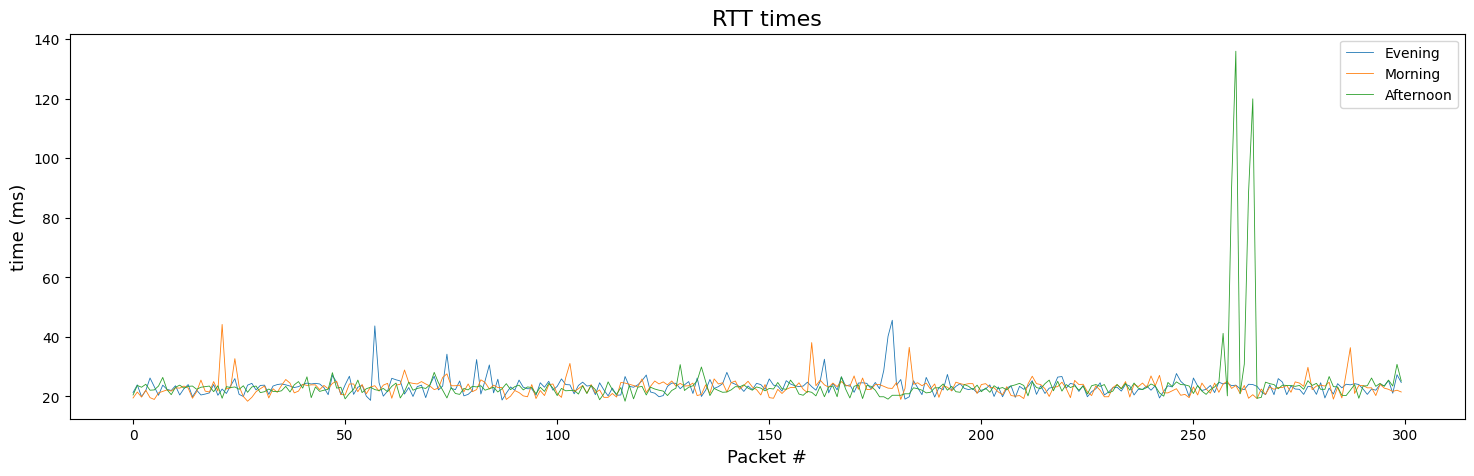
\includegraphics[width=1\textwidth]{time_RTT_hours_april_2.png}
                \caption{\small ping RTTs (PV) on April, 2 and April, 3}
                \label{fig:RTTs_PV}
        \end{figure}

\begin{multicols}{2}

\noindent
The first thing coming to our eyes is the presence of a spike toward the end in the blue line 
that took place in the last part of the afternoon ping measurement. To try to understand the causes was analyzed the traffic 
for that time using the wireshark (.pcapng) proper record, however no anomalous traffic was found, only the classic ICMP packets used by ping were captured.
A deeper control that can be performed to try to find out the reasons of the spike is a check on the traceroute (figure \ref{fig:Scatter_april_2}). Once again 
in the afternoon the RTT behavior seems normal and doesn't provide useful information to explain the spike causes. The cause can be that the path from vantage point to target
can change and since the traceroute was not executed in the exact moment of the ping, it might have not captured the exact moment of the issue.
Another possible explanation to the spike is a temporary issue somehow related to a specific hostname configuration.
The target servers involved in the spike are those in table \ref{tab:anomalous_RTT} and can be themselves object of a monitoring project, using active and passive 
tools by the servers administrator, with the aim of discovering possible issues. The spike justification can also be related to a temporary network 
congestion on any nodes on the specific path taken in that situation. 
In general to infer the causality in a network is a very difficult task, and requires
measurements extended in time and across different strategical nodes, together with all the permissions to access the servers and use passive tools on them.\\

        \begin{table}[H]
                \centering
                \caption{\small Hostnames with anomalous RTT}
                \vspace{0.3cm}
                \begin{tabular}{|c|c|c|} \hline
                \textbf{Packet N.} & \textbf{RTT (ms)} & \textbf{RTT (ms)}\\ \hline
                260 & apple.de & 136.0 \\ \hline
                264 & brkgls.com & 120.0 \\ \hline
                259 & seminars.apple.com & 90.2 \\ \hline
                263 & apple.com.mx & 88.5 \\ \hline
                \end{tabular}
                \label{tab:anomalous_RTT}
        \end{table}

\noindent
Since the spike is a very isolated case we can disregard it for the goal of the analysis. Doing that it is possible to notice in figure \ref{fig:RTTs_PV_hours}
that the blue line is almost everywhere slightly higher than the orange one. Figure \ref{fig:Boxplot_full_PV} provide another representation of the same phenomenon.

        \begin{figure}[H]
                \centering
                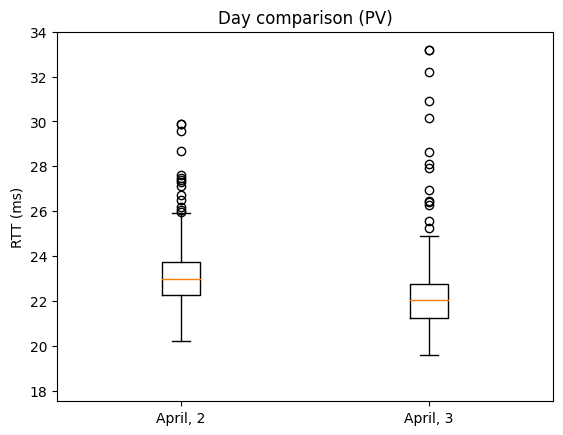
\includegraphics[width=0.48\textwidth]{Boxplot_full_PV_nospike.png}
                \caption{\small ping RTTs (PV) on April, 2 and April, 3}
                \label{fig:Boxplot_full_PV}
        \end{figure}

\noindent
Even if the difference is small this can indicate a higher traffic level on the weekend day (April, 2).
At the end what comes out this first analysis, is that the latency is slightly higher on April, 2 rather than on April, 3 and this could be related
to an higher network usage. The data in table \ref{tab:speedtest_table} support this hypothesis since the average download and upload speed on sunday 2 April
was smaller respect to Monday 3 April. Also the packet loss rate is a signal of network congestion because an higher loss rate can be related to an higher traffic level.
In table \ref{tab:lost_packets_table} it is possible to see that on sunday the loss rate was higher on average.\\
A last brief analysis is done looking inside each day. In figure \ref{fig:Boxplot_hours_2_PV} and figure \ref{fig:Boxplot_hours_3_PV} are shown the latencies 
at a hours level. What they show is that on April, 2 the latency remained constant along the day and this is reasonable because it was a sunday, so people 
used the network all along the day. On the other side on April, 3 the situation is similar with a slightly higher median latency on afternoon.

        \begin{table}[H]
                \centering
                \caption{\small Loss rate}
                \vspace{0.3cm}
                \begin{tabular}{|c|c|}
                \hline
                \textbf{Session} & \textbf{Loss rate}\\ \hline
                April, 2 Morning & 5.31 \\ \hline
                April, 2 Afternoon & 3.88 \\ \hline
                April, 2 Evening & 3.81 \\ \hline
                April 3, Morning & 2.18 \\ \hline
                April 3, Afternoon & 1.56 \\ \hline
                April 3, Evening & 3.43 \\ \hline
                \end{tabular}
                \label{tab:lost_packets_table}
        \end{table}

\end{multicols}

        \begin{figure}[H]
                \centering
                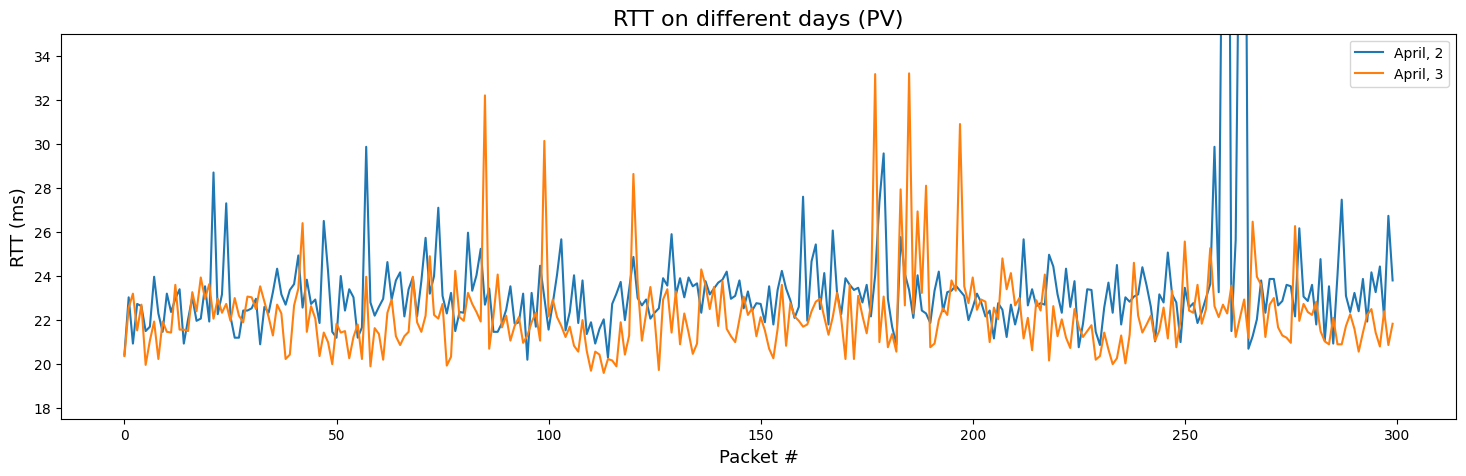
\includegraphics[width=1\textwidth]{RTT_PV_comparison.png}
                \caption{\small Magnified ping RTTs from PV on April, 2 and April, 3}
                \label{fig:RTTs_PV_hours}
        \end{figure}

\begin{multicols}{2}

        \begin{figure}[H]
                \centering
                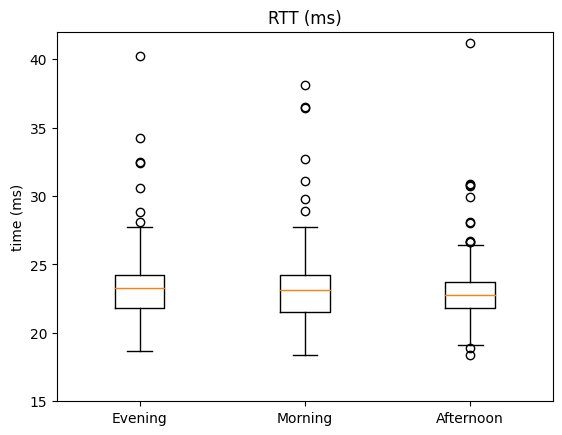
\includegraphics[width=0.48\textwidth]{Boxplot_hours_PV_april_2.png}
                \caption{\small ping RTTs (PV) on April, 2}
                \label{fig:Boxplot_hours_2_PV}
        \end{figure}
        
        \begin{figure}[H]
                \centering
                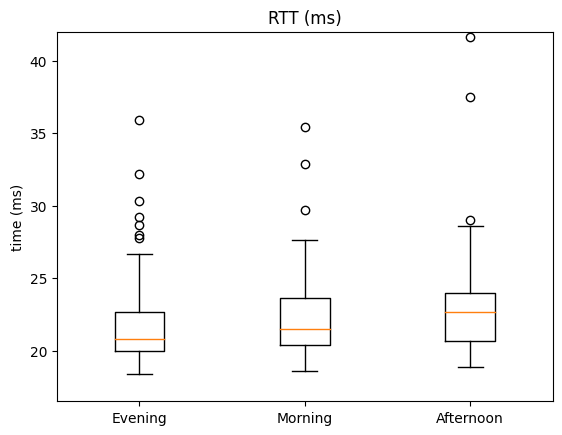
\includegraphics[width=0.48\textwidth]{Boxplot_hours_PV_april_3.png}
                \caption{\small ping RTTs (PV) on April, 3}
                \label{fig:Boxplot_hours_3_PV}
        \end{figure}

\subsubsection*{Traceroute analysis}
Ping provides information about the RTT between the vantage point and the target, so it doesn't provide any information about the path the packet follows.
This can be a problem because in case of an issue we cannot know whether the issue is related to the target server or to any of the nodes on the path
connecting it with the source. For this reason it is useful to use traceroute. This tool provides information about the path the packet takes, that way 
it is possible to investigate the situation of each single hop and eventually find out the cause of the problems. In figure \ref{fig:Scatter_april_2} and
figure \ref{fig:Scatter_april_3} are shown the traceroute results for the two days of measurements.\\
Since traceroute sends sequences of three packets each one, the time on y axis is the mean of the three packets RTTs. \\
To interpret figure the following observation must be considered:\\
- When on the same hop there are more points with the same colors, means that on that hop 
the target received reply from different routers that was at the same distance from the vantage point. \\
- When a point of a color is missing from a specific hop means that no packets among the three received reply for that hop. This happened because that path 
was blocked for many different reasons.\\
Comparing the two figures we can see two main things: the first one is that on April, 2 there is a slightly higher variance in the time. This supports
what the ping test showed, on that day there was an higher traffic on the network. The second thing is that in both of them there
is a clear common pattern: the first hop is characterized by the lowest time, between 2 and 8 the times are very similar and in the last three hops there
is an increasing in time for the replies. The reason of that pattern is that the first hop is the local router and it is close to the source. Between
the hops 2 and 8 the packets follow almost always the same path and they are under the ISP (Vodafone IT) network of the vantage point. On hop 9 the network 
changes and the situation stays the same until the target server is reached. Most of time the network of the last three hops is German network, with the 
hop 9 located in Frankfurt, however it is not a stable situation since happened the servers were located in UK or France.    

        \begin{figure}[H]
                \centering
                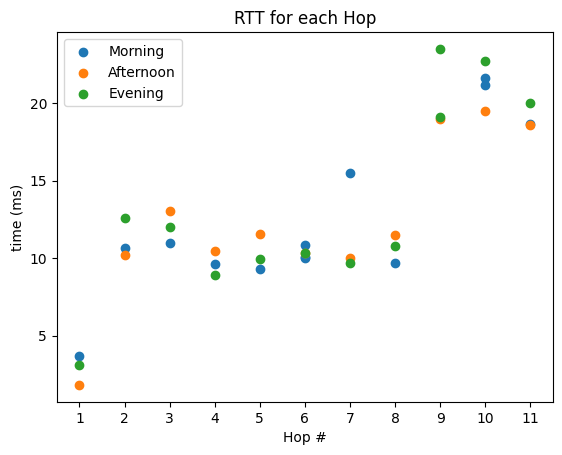
\includegraphics[width=0.48\textwidth]{scatter_april_2.png}
                \caption{\small Traceroute RTTs (PV) on April, 2}
                \label{fig:Scatter_april_2}
        \end{figure}

\subsubsection{Project part 2: new vantage point}
In this section there is a brief comparison between ping, traceroute and mtr results from a different vantage point. The vantage point is Ponte Caffaro (BS) and
the results are collected on evening during the week. 
To be consistent, the data from the new vantage point are compared with the data collected on evening during the week in Pavia (April, 3).\\
The ping result in figure \ref{fig:ping_BSvsPV} shows a huge difference between the two vantage points. The RTTs obtained from Ponte Caffaro (BS) are much 
bigger than those collected in Pavia and they have an higher variance as well.\\
A first motivation is that the type of internet connection in the 
two places is different: in Pavia the connection exploits a FTTH (Fiber To The Home) technology while in Ponte Caffaro is used a 4G router. 
The first is more reliable and faster since makes use of physical cable connection to vehicle signal, while the second one uses radio waves so it is
more unstable. It is also important to underline that while the fiber connection is provided by Vodafone IT, is WindTre the ISP providing the 4G connection 
in Ponte Caffaro. To have a more clear view over the causes leading to that big difference in the RTT, in figure \ref{fig:trace_BSvsPV} is showed a traceroute comparison.

\end{multicols}

        \begin{figure}[H]
                \centering
                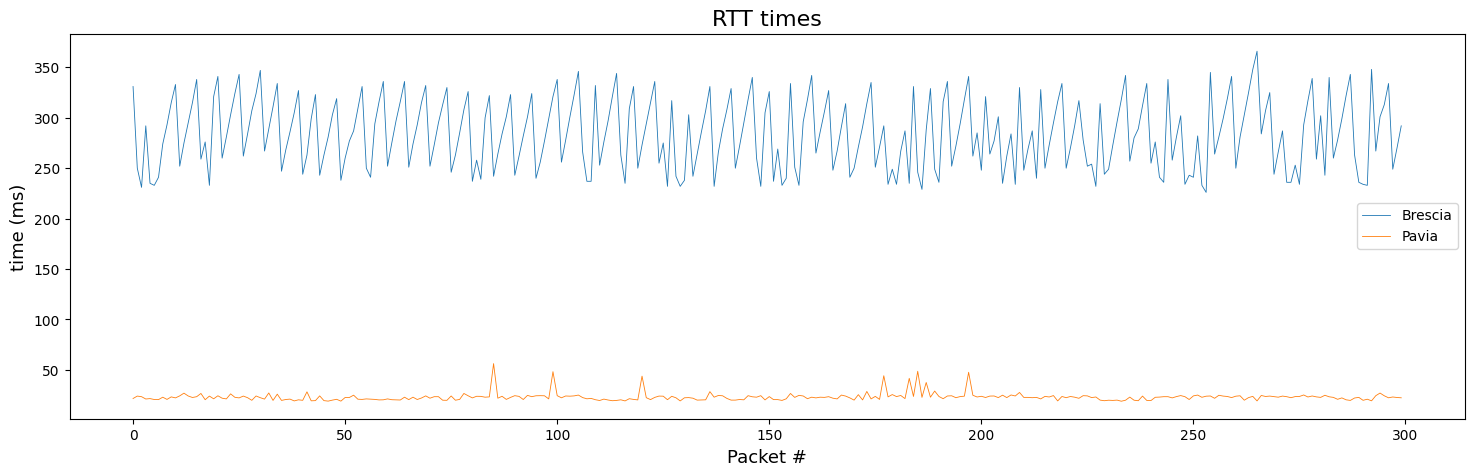
\includegraphics[width=1\textwidth]{Ping_BSvsPV.png}
                \caption{\small Ping RTTs (PV) vs (BS)}
                \label{fig:ping_BSvsPV}
        \end{figure}

\begin{multicols}{2}


        \begin{figure}[H]
                \centering
                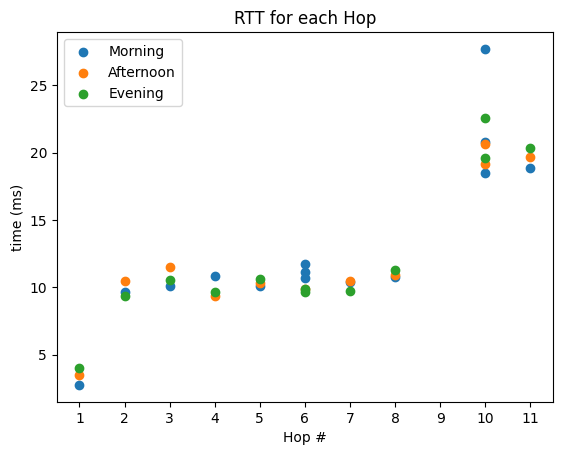
\includegraphics[width=0.44\textwidth]{scatter_april_3.png}
                \caption{\small Traceroute RTTs (PV) on April, 3}
                \label{fig:Scatter_april_3}
        \end{figure}

        \begin{figure}[H]
                \centering
                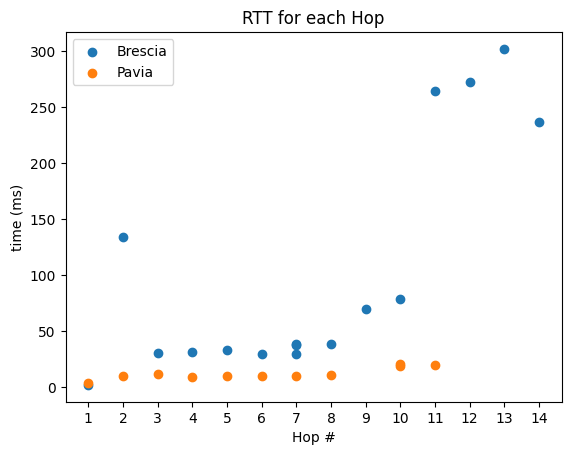
\includegraphics[width=0.44\textwidth]{Traceroute_BS_PV.png}
                \caption{\small Traceroute RTTs (PV) vs (BS)}
                \label{fig:trace_BSvsPV}
        \end{figure}


\noindent
The path, as expected, is different in the two situations, since the blue one takes 14 hops to reach the destination \textit{Apple.com} while 
the second one just 11 hops. 
The trend is similar because there are the middle hops with an almost constant latency, while the last hops are characterized by an higher latency, but let's analyze
deeper each single hop. The first one has a very low latency because, once again, it is the local router. The second one has an high latency and this is because
the packet has to pass through the air (due the 4G connection) to reach the third hop. Between hops 3 and 8 the packet is moving inside the WindTre network and, it is
interesting to see that, even if the latency is stable, it is higher than the one of the Vodafone network. In hop 9 and 10 there is a small increasing and this
is due to the passage from the local ISP network to \textit{liquidtelecom}. Inside this latter the packet moves from Frankfurt (hop 8) to Marseille and then
to Johannesburg (hop 11, 12, 13). This explains the higher latency, since packet probably crossed the ocean.\\
So, what justify the high latency saw in figure \ref{fig:ping_BSvsPV} is mainly the fact that from Ponte Caffaro the packet goes across the ocean. The high
variance is instead justified by the second hop. In figure \ref{fig:BS_StDev} is showed the standard deviation for each hop. The data were obtained
using \textit{mtr} command for 100 packets. It is clear that the second hop is characterized by an higher variance that influences the global variance of the ping result above. 
For completeness in table \ref{tab:BS_path} there is a full representation of the data coming from the \textit{mtr} execution. The fields are the 
distance between the vantage point and the specific node, the IP address together with hostname for the most relevant node, and some statistics about the 100
sent packets.

        \begin{figure}[H]
                \centering
                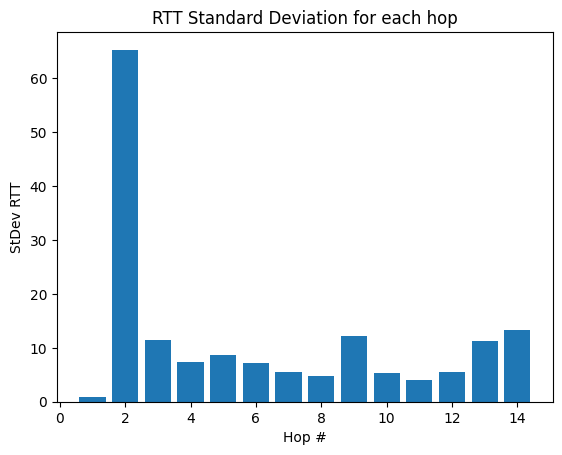
\includegraphics[width=0.48\textwidth]{BS_StDev.png}
                \caption{\small Traceroute RTTs (PV) vs (BS)}
                \label{fig:BS_StDev}
        \end{figure}

\end{multicols}
        
        \begin{table}[H]
                \centering
                \caption{\small Route details}
                \vspace{0.3cm}
                \begin{tabular}{|c|l|c|c|c|c|c|}
                \hline
                    \textbf{Hop} & \textbf{IP} & \textbf{Loss\%} & \textbf{Avg} & \textbf{Best} & \textbf{Worst} & \textbf{StDev} \\ \hline
                    1 & 192.168.1.1 & 0.0\% & 2.7 & 1.7 & 8.4 & 0.8 \\ \hline
                    2 & 172.16.142.129 & 0.0\% & 70.5 & 29.0 & 243.2 & 65.3 \\ \hline
                    3 & 172.16.142.44 & 0.0\% & 35.5 & 24.9 & 167.0 & 11.5 \\ \hline
                    4 & 172.16.14.52 & 0.0\% & 31.8 & 25.5 & 91.3 & 7.3 \\ \hline
                    5 & 151.6.92.115 & 0.0\% & 34.5 & 25.5 & 70.0 & 8.7 \\ \hline
                    6 & 151.6.92.34 & 0.0\% & 33.1 & 26.1 & 65.8 & 7.1 \\ \hline
                    7 & rmid-t02-miot-t02-po01.wind.it & 0.0\% & 31.9 & 25.7 & 55.6 & 5.5 \\ \hline
                    8 & 151.6.7.239 & 0.0\% & 32.3 & 25.5 & 54.3 & 4.7 \\ \hline
                    9 & decix-frankfurt.liquidtelecom.net-(80.81.193.228) & 0.0\% & 59.6 & 51.6 & 119.5 & 12.1 \\ \hline
                    10 & hu-0-0-0-2.lfr-p1-mrs.liquidtelecom.net-(5.11.12.30) & 0.0\% & 67.7 & 61.6 & 85.9 & 5.3 \\ \hline
                    11 & hu-0-1-0-1.lza-p3-jhb.liquidtelecom.com-(5.11.12.112) & 0.0\% & 227.8 & 222.0 & 238.9 & 4.0 \\ \hline
                    12 & hu-0-0-0-1.lza-p4-jhb.liquidtelecom.net-(41.175.242.17) & 0.0\% & 229.5 & 221.6 & 247.8 & 5.6 \\ \hline
                    13 & 41.175.246.13 & 0.0\% & 221.1 & 209.7 & 420.3 & 11.2 \\ \hline
                    14 & apple.com.sg-(17.253.144.10) & 4.0\% & 230.6 & 221.6 & 348.1 & 13.3 \\ \hline
                \end{tabular}
                \label{tab:BS_path}
            \end{table}
\newpage
 \begin{multicols}{2}
                
\subsubsection{Tools used and Quality of Measurements}
In this section there is a brief explanation about the used commands and how they works.

\subsubsection*{Ping}
\small\textbf{Goal}: ping is an active monitoring tool used to obtain the latency between two nodes of a network to test and debug it.\\
\small\textbf{How it works}: Ping is executed by one of the two nodes, the vantage point. During the execution, ping sends ICMP packets with variable payload
to the other, the target. When the target gets the packet it answer with an ICMP ECHO REPLY message and the latency (RTT) is measured as the time spent between the
departure (ICMP ECHO) of the packets and the reply.\\
\small\textbf{Drawbacks}: The main problem of the ping is that it doesn't provide information about the path. For this reasons it is impossible
to detect whether there is a network congestion and why the target is unreachable, since the problem can be in the path and not in the target. It is also important
to underline that the ping value is strongly affected by distance between the nodes and by the mean used for transmitting the signal (air or cable).\\
\small\textbf{Command used}: The command used in this project for the ping is: 
\begin{center}\textit{'ping  -c 320  apple.com  \(>>\)  filename.csv '} \end{center}
Where the \textit{'-c'} option set the number of packets to be sent and the \(>>\) symbol stores in the specified csv file the result.

\subsubsection*{Traceroute}
\small\textbf{Goal}: traceroute is an active monitoring tool used to discover the network topology between two nodes of a network.\\
\small\textbf{How it works}: vantage point executes traceroute and during the execution sequences of 3 packets are generated. To each sequence is
assigned a TTL value in the header that counts the maximum number of hops a packet can pass through. Whenever a router receives a packet
it decreases the TTL by one and checks its value: if TTL = 0 a ICMP reply \textit{'TIME EXCEEDED!'} is sent back to the source, if TTL != 0 
the packet is forwarded to the next hop. When the final target s reached a ICMP reply \textit{'PORT UNREACHABLE'} is sent to source. In this way, by setting
the first sequence with TTL = 1, the second with TTL = 2 and so on, it is possible to get the path followed by the packets and the RTT of each single hop.
It is important to notice that traceroute can send packets using different protocol (ICMP, UDP and TCP). The reply is always a ICMP reply.\\
\small\textbf{Drawbacks}: The problems of traceroute are related to the non stability in the taken route. There can be three situations:\\
- asymmetric path: due to congestion the departure path and the return path can be different, so we don't see the correct RTT.\\
- unstable path: due to congestion or failures the path can change from one packet to the other, so the order in which we discover the hop can change
and so we cannot discover the actual network topology.
- blocked path: due to many reasons a path can be blocked, so the packets are discarded and no reply is received for them. This is a problem that could
happen using the UDP protocol.\\
All these problems must be taken into consideration in the analysis. Because of them it is difficult to get to a correct identification of the 
factor causing any possible issue just by using traceroute and many other tools must be used to properly asses the network status.
\small\textbf{Command used}: The command used in this project for the traceroute is: 
\begin{center}\textit{'traceroute  apple.com  \(>>\)  filename.csv '} \end{center}
Where the absence of protocol specifications means that the standard UDP protocol is used. When the traceroute is used with the TCP protocol 
\textit('-T') a bug occurs and the target seems to be just 1 hop far from the vantage point, no matter how actually distant it is.

\subsubsection*{Speedtest}
\small\textbf{Goal}: speedtest is an active monitoring tool used to obtain information about the network speed.\\
\small\textbf{How it works}: When speedtest is executed an artificial traffic is generated from the source to the target. This latter is composed by 
downloads, uploads and ping tests. From this traffic it is possible to measure the network bandwidth in download and upload, the ping and the jitter.
The target server is usually chosen by the speedtest looking at the ping and taking the one with the smallest latency. However it can be specified also 
byt he user manually.\\
\small\textbf{Drawbacks}: The problem of the speedtest is that the results are influenced by many factors like, traffic, weather, distance between target and
vantage point. To improve reliability of the results is important to repeat the test multiple times and averaging the results.\\
\small\textbf{Command used}: The command used in this project for the speedtest is: 
\begin{center}\textit{'speedtest-cli  --secure'} \end{center}
Where the \textit{'--secure'} option impose to execute the speedtest with a target server that support secure HTTPS connection.


\subsubsection*{Mtr}
\small\textbf{Goal}: mtr is an active monitoring tool used to obtain information about the network latency and topology.\\
\small\textbf{How it works}: mtr is basically a combination of ping and traceroute. When it is running it generates sequences of packets each one with
TTl value as traceroute. It uses the strategy of this latter to discover network topology, however it goes on sending packets so it also provides
statistics about the latencies in each hop. An example of the mtr statistics in reported in table \ref{tab:BS_path}.\\
\small\textbf{Drawbacks}: The problems are those already seen for ping and traceroute.\\
\small\textbf{Command used}: The command used in this project for the mtr is: 
\begin{center}\textit{'sudo  mtr  --report-wide  -c 100  apple.com  \(>>\)  filename.csv'} \end{center}
Where the \textit{'--report-wide'} option specify the output format of the mtr command to display the final statistics and the hostname of the hops. The 
\textit{'-c'} option specifies the number of packets to be sent for each hop and the last part is used to store the results in the csv file.

\subsubsection*{Top}
\small\textbf{Goal}: top is an passive monitoring tool used to obtain information about the infrastructure resources status.\\
\small\textbf{How it works}: It provides information about CPU usage, mem usage, active processes and their resources consumption.\\
\small\textbf{Command used}: The command used in this project for the top is: 
\begin{center}\textit{'top'} \end{center}

\subsubsection*{Wireshark}
\small\textbf{Goal}: wireshark is an passive monitoring tool, in particular it is a sniffer used to collect all the information about the traffic
exchanged over the network.\\
\small\textbf{Command used}: The command used in this project for wireshark is:
\begin{center}\textit{'sudo wireshark'} \end{center}



%----------------------------------------------------------------

\subsection{Conclusions}
Project part 1:\\
\textbf{Goal}:
the goal of the first part was to investigate the connectivity and stability of the network connecting the vantage point in Pavia and the target server and
understanding the differences between a normal week day and a weekend day.
\\
\textbf{Conclusions}: 
as regard the network the project showed the complexity of the Apple infrastructure, which is composed by many machines, located in different places all around the world.
All of them are identified by the same IP, exploiting the \textit{host aliasing} DNS service and all of them redirect to a specific section the official Apple website.
The path to the server is stable and all the traffic passes through a Neutral Access Point in Milan, where the traffic switches from the ISP 'Vodafone' to 'Level 3 Parent, LLC'.
The network behavior was normal except for a spike in the RTT on Sunday April, 2 on afternoon. The hostname related to the anomalous behavior were identified and
reported in table \ref{tab:anomalous_RTT}. No particular traffic was found by Wireshark and the spike reasons are probably related to a network congestion
on any of the nodes of the taken path of the packets. According to table \ref{tab:apple-websites-rtt} there are hosts frequently slower than the others, but 
the reasons can be many and were not identified.\\
As regard the impact on a weekend day it came up that on Sunday the latency was higher on average and it remained constant during the whole day. No specific nodes
were responsible, the increase in latency was evenly distributed across them. On monday there was an higher latency on afternoon. In conclusion, the difference
in latency was very small in absolute term, so the results showed no significant impact of the weekend day on the network in the period of test April, 2 and April, 3.\\
\\
\\
Project part 2:\\
\textbf{Goal}: 
the goal was to investigate how changing the vantage point and its connection specifics would have changed the results, keeping the \textit{apple.com} server as target.
\\
\textbf{Conclusions}: 
the results as expected showed higher latency and instability for the 4G connection. In particular the route to the second hop was the most problematic and
responsible for the high variance of the results. 
This is because the signal had to pass trough the air using radio waves to reach the next hop. An interesting situation came up comparing the latencies of the path inside the
two ISP. Vodafone showed a lower latency than WindTre as long as the packets traveled inside their networks.\\
The path followed by the packets from Ponte Caffaro to apple.com changed as expected. The first part was similar to Pavia, the packet traveled to Milan, where 
it switched from 'WindTre' ISP network to the ISP 'Liquid Telecommunications Ltd'. The last part was different because packets are sent across the ocean to Johannesburg
and this explained the high total latency value from Ponte Caffaro.\\
In conclusion two of the causes of the bad results in latency got in Ponte Caffaro were the 4G connection and the different path taken that crossed the ocean.
\newpage






%###############################################################




%----------------------------------------------------------------

%-----------------------SECOND LAB-------------------------------

%----------------------------------------------------------------

\section{The Domain Name System}
%what is the DNS: when it is used, lookup phase, structure, db contents, how it works.

\subsection{Introduction}
The second lab activity was about the practical implementation of many tools used to perform queries and test the performance of the DNS.
The goal was to understand how the DNS works, what is the role of the different components and what is the meaning of the different DNS records.
As tools to perform queries we saw \textit{'dig', 'host', 'nslookup' and 'jwhois'} and we tried to use them across different DNS servers to see
whether differences were presents between them. As performance tools we tried \textit{'dnsperf', 'dnsping', 'dnstraceroute' and 'dnseval'}. For these latter
as well different name servers were tested to check for the differences.\\
To practically use the introduced tools, in the next sections is proposed a DNS project composed by two sections:\\
1. Active experiments in which various DNS servers are queried.\\
2. Performance experiments in which some diagnostic tools are used to check the behavior of different Name Servers.\\ 
Both sections are structured in single experiment, each one faced using a 
question-answer format, which allow for an easier understanding of the particular DNS feature and the tools used.



%----------------------------------------------------------------

\subsection{Methodology}

Each of the experiment could become a project itself and it could be managed using the \textit{'Why, Which, What, Where, How, When'} methodology. Since the goal
of this project is to understand the DNS in general and provide a panoramic view about how it works, the adopted methodology is more simple and can be resumed in 3 main points:\\
1. Select a list of DNS servers to be used for the experiments. The choice criteria is the popularity of the company providing the service.\\
2. Introduce the specific question and briefly explain it.\\
3. Perform the experiment and answer to the question.\\
\\
%insert the used tools and what they are used for
The tools used are:\\
- \textit{'dig'}: a tool used to perform DNS queries and getting information about many resource records.\\
- \textit{'whois'}: used to retrieve information about a domain like the owner, the registrar and the creation date.\\
- \textit{'dnstraceroute'}: used to trace the path followed by the DNS resolution process.\\
- \textit{'dnseval'}: used to evaluate the performance of a list of DNS servers on the same set of queries.\\


%----------------------------------------------------------------

\subsection{Experimental Setup}
%describe the chosen DNS servers
The DNS server used are reported in table \ref{tab:dns_servers} together with some specifications. Other servers used for specific experiments are reported in the related section
in table \ref{tab:dns_location}
        
        \FloatBarrier
        \begin{table*}[htbp]      
                \centering
                \caption[\small DNS Servers used for the experiments]{\small DNS Servers used for the experiments}
                \vspace{0.3cm}
                \begin{tabular}{|l|l|c|c|c|}
                \hline
                \textbf{DNS Server} & \textbf{Company} & \textbf{Location} & \textbf{IPv4} & \textbf{IPv6} \\ \hline
                \textit{dns.google} & Google & Global (distrib. network) & 8.8.8.8 & 2001:4860:4860::8888 \\ \hline
                \textit{one.one.one.one} & Cloudflare & Global (distrib. network) & 1.1.1.1 & 2606:4700:4700::1111 \\ \hline
                \textit{dns.opendns.com} & Cisco & Global (distrib. network) & 208.67.222.222 & 2620:119:35::35 \\ \hline
                \textit{dns9.quad9.net} & Quad9 & Global (distrib. network) & 9.9.9.9 & 2620:fe::fe \\ \hline
                \textit{ipv36.unipv.it} & UniPV & Pavia (IT) & 193.204.35.27 & - \\ \hline 
                \textit{a16-64.akam.net} & Harvard & Cambridge (US) & 23.211.132.64 & 2600:1406:1b::40 \\ \hline
                \textit{ns1.iransamaneh.com} & - & Iran & 94.182.146.2 & - \\ \hline
                \textit{ns1.headgear.org} & Spec & - & 192.3.51.204 & - \\ \hline
                \textit{ns1-39.azure-dns.com} & Microsoft & Redmond (WA) & 150.171.10.39 & 2603:1061:0:10::27 \\ \hline
                \end{tabular}
                \label{tab:dns_servers}
        \end{table*}
\noindent
All the experiments were conducted using a Virtual Machine (VM) equipped with Ubuntu 22.04 LTS, running on a Macbook Pro 14' with 16GB of RAM and 512GB of SSD.\\
The internet connection was a FTTH provided by 'Vodafone IT' and the computer was connected to the router in a Wi-Fi mode. All the experiments were conducted on April, 21 and April, 22 on morning
from Pavia (IT).

\subsection{Experimental Execution and Results}

%insert the questions, explanation and answers (FULL FOCUS HERE)

\subsubsection*{Active experiments}

1. Query the DNS to obtain the IP addresses of \textit{achille.unipv.it} and of another hostname in the TLD domain it. Are the answers authoritative? Why?\\
To query the DNS to obtain the IP address it is possible to use the command \textit{'dig'} and to understand if an answer is authoritative or not it is possible to check 
the \textit{'flags'} field in the output data looking for the string \textit{'aa'}. In figure \ref{fig:dig_output} is shown the output of a dig command.
 The syntax of the command used is \textit{'dig @[DNS\_server] [hostname] -t A'} where 
the content of the squared brackets can be varied. The results are inserted in table \ref{tab:quest_1}.

        \begin{figure}[H]
                \centering
                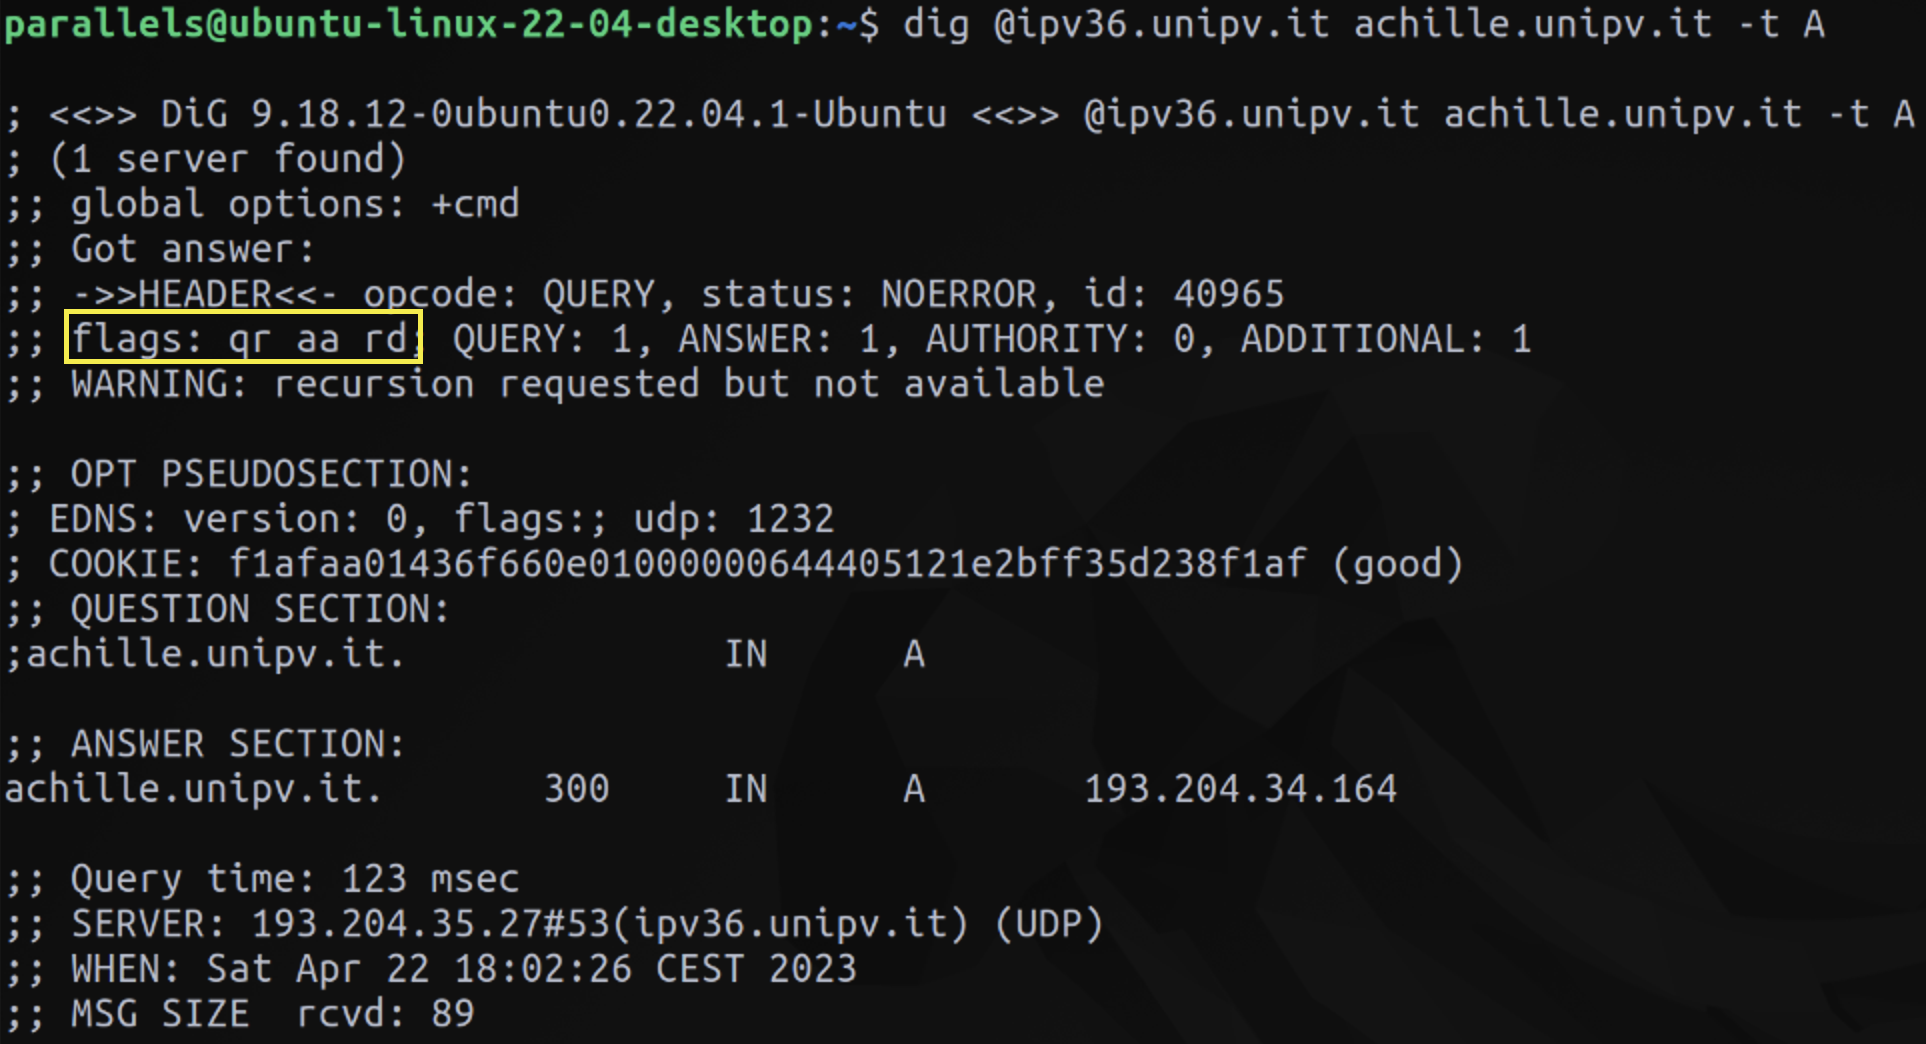
\includegraphics[width=0.48\textwidth]{dig_screen.png}
                \caption{\small Example of 'dig' command output}
                \label{fig:dig_output}
        \end{figure}


        \begin{table}[H]
                \centering
                \caption{\small Flags field for the queries}
                \vspace{0.3cm}
                \begin{tabular}{|c|c|c|}
                \hline
                \textbf{NS-IP} & \textbf{achille.unipv.it} & \textbf{www.apple.it} \\ \hline
                {8.8.8.8} & qr rd ra & qr rd ra \\ \hline
                {1.1.1.1} & qr rd ra & qr rd ra \\ \hline
                {208.67.222.222} & qr rd ra & qr rd ra \\ \hline
                {9.9.9.9} & qr rd ra & qr rd ra \\ \hline
                {193.204.35.27} & \cellcolor{cyan} qr aa rd & qr rd \\ \hline
                \end{tabular}
                \label{tab:quest_1}
        \end{table}
\noindent
From table \ref{tab:quest_1} it is possible to see that the only authoritative answer is the one provided by the name server 193.204.35.27 for the hostname
\textit{'achille.unipv.it'}. This is because it is the IP of \textit{'ipv36.unipv.it'} which is the official name server of the University of Pavia and the hostname is a subdomain of the domain.
So, the name server is the proprietary of the record I asked for. All the other answers are not authoritative because the name server queried is not the owner of the record. 
In this case the other name servers are recursive name servers that ask other NSs about the query and just provide the final answer.\\
\\
\noindent
2. Query the DNS to obtain the name(s) of the mail servers associated with the domain \textit{'universitadipavia.it'} and \textit{'harvard.edu'}. How many servers provide this service? Is there anything 
specific associated with these RRs?\\
\\
The command used to query the DNS is again dig. The syntax is \textit{'dig @[DNS\_server] [hostname] -t MX'}. The results are inserted in table \ref{tab:quest_2}.

        \begin{table}[H]
                \centering
                \caption{\small Number MX records associated with \textit{'universitadipavia.it'} and \textit{'harvard.edu'}}
                \vspace{0.3cm}
                \begin{tabular}{|c|c|c|}
                \hline
                \textbf{NS-IP} & \textbf{...dipavia.it} & \textbf{harvard.edu} \\ \hline
                {8.8.8.8} & 7 & 2 \\ \hline
                {1.1.1.1} & 7 & 2 \\ \hline
                {208.67.222.222} & 7 & 2 \\ \hline
                {9.9.9.9} & 7 & 2 \\ \hline
                {193.204.35.27} & \cellcolor{cyan} 7 & \cellcolor{red} 0 \\ \hline
                {23.211.132.64} & \cellcolor{red} 0 & \cellcolor{cyan} 2 \\ \hline
                \end{tabular}
                \label{tab:quest_2}
        \end{table}
\noindent
The cells red colored are those related to the name servers that didn't provide any MX RR. The cells cyan colored are those related to the name servers that provided an authoritative
answer for the requested records. This happens because 23.211.132.64 is the IP of the NS \textit{'a16-64.akam.net'} which is an official NS for the \textit{'harvard.edu'} domain, so it is
the owner of the records MX for that domain. The same happens with the IP 193.204.35.27 for the MX records of \textit{'universitadipavia.it'}. This means that the NS associated with the domain \textit{'unipv.it'} (which are 2)
are the same that are associated to \textit{'universitadipavia.it'}. All the other name servers, as expected since they are recursive NS, provided the queried records. 
An interesting thing to observe is that the order in which the mail servers are provided changes every time. This is due to a the implementation of a load balancing mechanism that 
changes each time the order in which the MX are provided to distribute the work across them. (The chosen mail server is always the first of the list).  \\
\\
\noindent
3. Query the DNS to obtain the IP address of a Web server located outside Europe; is the answer authoritative? Why? How many RRs did you obtain? What is their type? 
Does the domain sign any RR type using DNSSEC?\\
\\
The web servers chosen are \textit{'www.spec.org'} and \textit{'www.yjc.ir'}. The command syntax is \textit{'dig @[DNS\_server] [hostname] -t A'} and it is possible to 
proceed as before to understand if the answer is authoritative or not. Since the results for the recursive name servers are the same, in table \ref{tab:quest_3_spec} and table \ref{tab:quest_3_yjc}
are reported only the results from 8.8.8.8 among them.

        \begin{table}[H]
                \centering
                \caption{\small Queries results for www.spec.org}
                \vspace{0.3cm}
                \begin{tabular}{|c|c|c|}
                \hline
                \textbf{NS-IP} & \textbf{flags} & \textbf{RR} \\ \hline
                8.8.8.8 & qr rd ra & CNAME, A \\ \hline
                193.204.35.27 & qr rd ra & - \\ \hline
                23.211.132.64 & qr rd ra & - \\ \hline
                192.3.51.204 & \cellcolor{cyan} qr aa rd & CNAME, A \\ \hline
                94.182.146.2 & qr rd & - \\ \hline
                \end{tabular}
                \label{tab:quest_3_spec}
        \end{table}

        \begin{table}[H]
                \centering
                \caption{\small Queries results for www.yjc.ir}
                \vspace{0.3cm}
                \begin{tabular}{|c|c|c|}
                \hline
                \textbf{NS-IP} & \textbf{flags} & \textbf{RR} \\ \hline
                8.8.8.8 & qr rd ra & CNAME, A \\ \hline
                193.204.35.27 & qr rd ra & - \\ \hline
                23.211.132.64 & qr rd ra & - \\ \hline
                192.3.51.204 & qr rd & - \\ \hline
                94.182.146.2 & \cellcolor{cyan} qr aa rd & CNAME, A \\ \hline
                \end{tabular}
                \label{tab:quest_3_yjc}
        \end{table}
\noindent
There are cells in which no RRs are inserted and this is due to the fact that the NS queried didn't provide any answer. This is the case of the NS of University of Pavia and Harvard (seen above)
that are neither recursive ones nor NS of the domain to which the queried hostname belongs. The same holds for the NS of \textit{'ycj.ir'} when queried about \textit{'www.spec.org'} and vice-versa.
Once again, the cyan colored cells are those in which the answer has been authoritative. In this case the reason is that 94.182.146.2 is the IP of \textit{'ns1.iransamaneh.com'} which is the 
NS of the domain \textit{'yjc.ir'} and it is the owner of the records A for \textit{'www.yjc.org'}. The IP 192.3.51.204 is the IP of \textit{'ns1.headgear.org'} which is the NS of the domain
\textit{'spec.org'}. In both cases the RRs received are two, the first one is a CNAME and the second one is an A type. This means that the hostname for which the query was submitted is an alias
of another hostname (provided in CNAME). In this situation a new query about this latter starts and eventually the IP is given.\\
To see if the domains signed anything using DNSSEC the command to use is \textit{'dig @[DNS\_server] [domain] +dnssec'}. In this case no answers are provided by both domains, so they don't
sign any RR using DNSSEC.\\
\\
\noindent
4. Query the DNS to obtain the IP addresses of the Name Servers of a company located outside Europe. How many queries did you execute? What type(s) of 
queries? How many Name Servers are associated with the company? Do they belong to the same domain? Can you identify the primary Name Server? Why?
Who registered the domain? When will it expire?\\
\\
The company chosen is Microsoft. A first approach that can be used to obtain the NS of the domain \textit{'microsoft.com'} is to replicate the behavior of a 
recursive name server (assuming no RR are present in cache). First of all with the \textit{'dig'} command we get the list of the root name servers. We take on of them and with the command \textit{'dig @[root\_ns] microsoft.com -t NS'}
we get the list of the NS associated with the TLD \textit{'.com'}. We take one of them and with the command \textit{'dig @[TLD\_ns] microsoft.com -t NS'} we get the list of the NS associated with
the domain \textit{'microsoft.com'}.\\
This approach is a pure didactic one since the list of the NS associated with the domain \textit{'microsoft.com'} can be directly obtained using the command \textit{'dig microsoft.com -t NS'} that 
asks the Local Name Server of our ISP to do the job for us. The results are in table \ref{tab:quest_4}.

        \begin{table}[H]
                \centering
                \caption{\small NSs list of microsoft.com}
                \vspace{0.3cm}
                \begin{tabular}{|c|c|c|}
                \hline
                \textbf{NS} & \textbf{IP} \\ \hline
                ns1-39.azure-dns.com. & 150.171.10.39 \\ \hline
	        ns2-39.azure-dns.net. & 150.171.16.39 \\ \hline
                ns3-39.azure-dns.org. & 13.107.222.39 \\ \hline
                ns4-39.azure-dns.info. & 13.107.206.39 \\ \hline
                \end{tabular}
                \label{tab:quest_4}
        \end{table}
\noindent
All the NSs belong to different TLDs and each time the query is performed the NS order changes thanks to the load balancing mechanism. To identify the primary name server is it possibile
to execute the command \textit{'dig microsoft.com -t SOA'} and look at the first value which is the primary name server name. In this case the primary NS is \textit{'ns1.39.azure-dns.com.'}.\\
To get information about the domain \textit{'microsoft.com'} it is possible to use the command \textit{'whois microsoft.com'}. The results are resumed in table \ref{tab:quest_4_whois}.

        \begin{table}[H]
                \centering
                \caption{\small Whois for microsoft.com}
                \vspace{0.3cm}
                \begin{tabular}{|c|c|}
                \hline
                \textbf{Whois} & \textbf{Value} \\ \hline
                Domain Name: & microsoft.com \\ \hline
                Registrar: & MarkMonitor, Inc. \\ \hline
                Registrant Organization: & Microsoft Corporation \\ \hline
                Registrant State/Province: & Washington \\ \hline
                Registered on: & 1991-05-02 \\ \hline
                Expires on: & 2024-05-03 \\ \hline
                DNSSEC: & unsigned \\ \hline
                \end{tabular}
                \label{tab:quest_4_whois}
        \end{table}
\noindent
A curious thing is that the field DNSSEC has the value \textit{'unsigned'} which means that the domain \textit{'microsoft.com'} doesn't sign any RR using DNSSEC.\\
\\
\noindent
5. Query one of the Name Servers identified in the previous experiment to obtain the IP address of the Name Servers of the domains unipv.it and 
cloudflare.com. How many IP addresses did you get? Why?\\
\\
The chosen NS is \textit{'ns1-39.azure-dns.com'} which is the primary NS of the domain \textit{'microsoft.com'}. The commands executed to answer the question are the following:\\
- \textit{'dig @ns1-39.azure-dns.com unipv.it -t NS'}.\\
- \textit{'dig @ns1-39.azure-dns.com cloudflare.com -t NS'}.\\
Both of them returned no answer, because they don't know about the domain \textit{'unipv.it'} and \textit{'cloudflare.com'} and they are not recursive.\\




\subsubsection*{Performance experiments}

1. Measure the performance of a Name Server when processing multiple queries. Did you notice any variability? Any expected/unexpected behavior? Does the 
performance depend on the transport protocol (i.e., UDP, TCP) or on usage of encrypted transmissions (i.e., DoT, DoH)? Does the performance vary when DNSSEC is enabled?\\
\\
To measure the performance of a NS when processing multiple queries it is possible to use the tool \textit{'dnseval'}. 
The command used is \textit{'dnseval -j [filename.json] -c 100 -f [DNS\_servers.txt] --[mode] -t A google.com'}
where \textit{'filename.json'} is the output file, \textit{'DNS\_servers.txt'} is the list of the DNS servers to use, \textit{'-c 100'} is the number of times the query 
is repeated and \textit{'mode'} is the protocol. The DNS server used is just the one provided by Google (8.8.8.8) and the 
protocols used are \textit{udp}, \textit{tcp}, \textit{dot} and \textit{doh}. To test the DNS server with DNSSEC, the option \textit{'--dnssec'} can be used.
The results are shown in figure \ref{fig:latency_8888}.\\

        \begin{figure}[H]
                \centering
                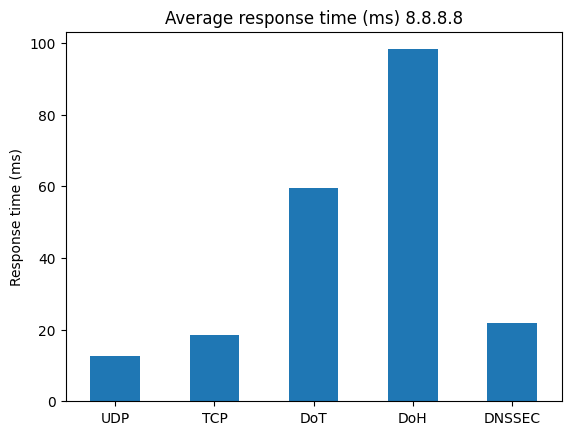
\includegraphics[width = 0.49\textwidth]{latency_8888.png}
                \caption{\small Google DNS latency}
                \label{fig:latency_8888}
        \end{figure}

\noindent
As expected the lowest latency is associated with the UDP protocol and all the others have an higher value. The highest values are associated with the DoT and DoH protocol. The reason is that
these protocols are encrypted and the encryption process takes time. In the case of TCP we have a slightly higher latency than UDP, because the communication is done using TCP
that requires a three way handshake to open the connection and takes time. As regard DNSSEC a clarification is needed: 
using \textit{-D} we are simply asking the DNS server to query the others name servers about the hostnames required, setting the DNSSEC flag in the query. The response
could be or not signed using DNSSEC, depending on whether the asked name server has or not the requested RR signed with DNSSEC. This situation can strongly affect the results. 
In our case no RR is signed with DNSSEC, so the increase in time is due to the configuration of the NS to manage the requests using DNSSEC and not to the actual decrypting process.\\
For completeness in figure \ref{fig:all_latency} are shown the results of the same experiment but using different DNS servers. The pattern is the same already described.\\

        \begin{figure}[H]
                \centering
                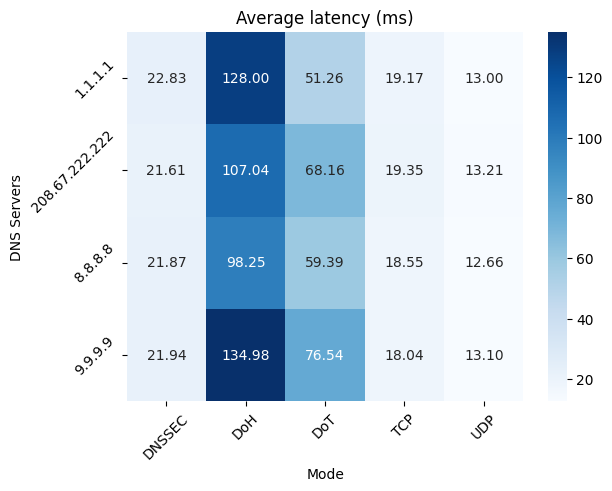
\includegraphics[width = 0.49\textwidth]{all_latency.png}
                \caption{\small DNS servers latency}
                \label{fig:all_latency}
        \end{figure}

\noindent
2. Measure the performance of different Name Servers when processing the same set of queries. Does the performance vary with the Name Server? Does it depend on the type of query or on the geographic 
location of the Name Server?\\
\\
To answer this question a set of DNS servers from various locations are used. All of them come from the website \textit{'https://public-dns.info'} and are listed in table \ref{tab:dns_location}. 
For each server the query to the hostname \textit{google.com} is executed 100 times for the types \textit{A}, \textit{SOA}, \textit{NS} and \textit{ANY}.

        \begin{table}[H]
                \centering
                \caption{\small DNS servers location}
                \vspace{0.3cm}
                \begin{tabular}{|c|c|}
                \hline
                \textbf{DNS-IP} & \textbf{Location} \\ \hline
                88.220.66.4 & Gmina Polaniec (PL) \\ \hline
                82.199.35.101 & Logrono (ES) \\ \hline
                185.218.125.68 & Dusseldorf (GE) \\ \hline
                98.33.182.119 & Kaysville (USA) \\ \hline
                210.237.36.39 & Kagoshima (JP) \\ \hline
                \end{tabular}
                \label{tab:dns_location}
        \end{table}

\noindent
The results related to the location comparison in figure \ref{fig:location_latency} show that the latency is strongly affected by the location of the servers. As expected the distance between the
client and the server affects the latency. The lowest values are associated with European server, while higher values are associated with the American server and the highest with the Japanese one.\\
As regard the impact that different types of queries has on the latency the results are shown in figure \ref{fig:type_latency}. The latency changes depending on the type of query. The lowest is related
to type A, while the type ANY is characterized by the highest latency. two reasons can be the larger amount of data provided by the type ANY and the usage of the TCP protocol for the 
communication.\\

        \begin{figure}[H]
                \centering
                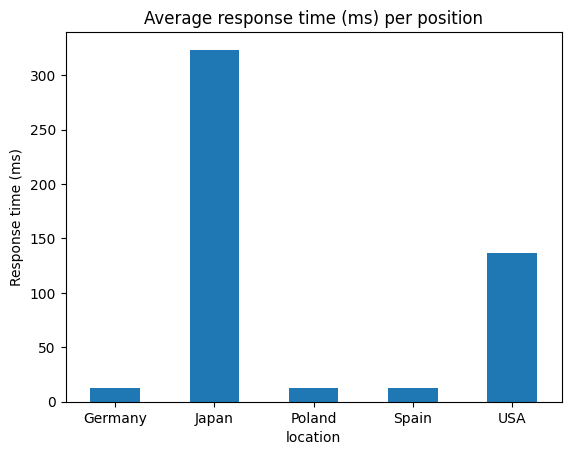
\includegraphics[width=0.49\textwidth]{location_latency.png}
                \caption{\small NSs latency (average among all the types)}
                \label{fig:location_latency}
        \end{figure}

        \begin{figure}[H]
                \centering
                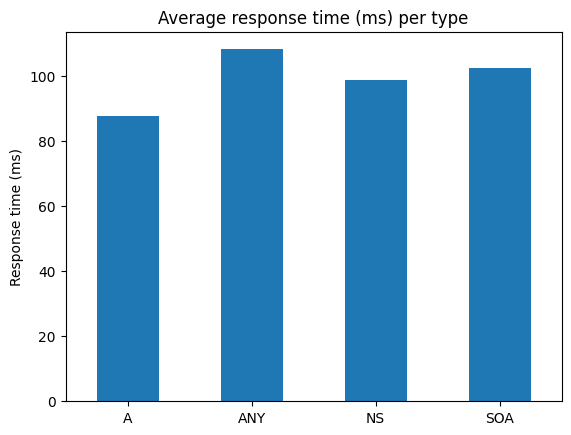
\includegraphics[width=0.49\textwidth]{type_latency.png}
                \caption{\small NSs latency (average among all the locations)}
                \label{fig:type_latency}
        \end{figure}
\noindent
Finally in figure \ref{fig:location_type_latency} is reported a full comparison involving all the different locations and types. The type A is still the one with the lowest latency
however, the type ANY in the European NS has a latency similar to the other query types. The result saw above in thus strongly influenced by the time from Japan and USA.\\
At the end we can say that the latency is strongly affected by both the location of the DNS server and the type of query.\\

        \begin{figure}[H]
                \centering
                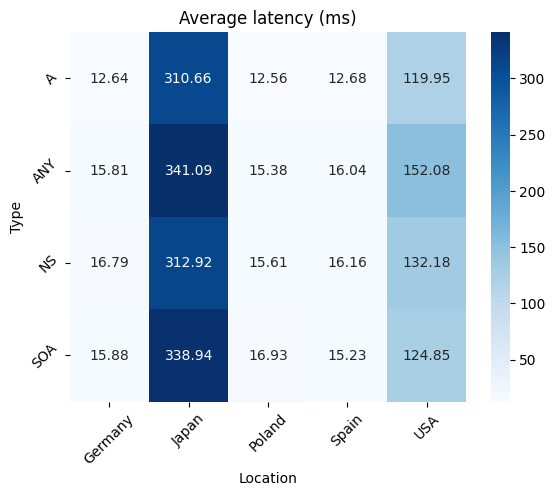
\includegraphics[width=0.49\textwidth]{location_type_latency.png}
                \caption{\small Location vs type latency }
                \label{fig:location_type_latency}
        \end{figure}
\noindent
3. Check the path followed by your queries using different Name Servers. Does the performance depend on the number of hops? Did you notice any expected/unexpected behavior?\\
To answer this question it is necessary to use the \textit{dnstraceroute} tool. The tool is used to trace the path followed by the DNS queries. The command used is \textit{'dnstraceroute -e -s [DNS\_server] -t A google.com'}
and the results are shown in figure \ref{fig:time_hops}. As expected the time time doesn't depend on the number of hops. In fact, even if it is true that the distance between the start point and the 
end point of a query strongly influences the time, the number of hops is not a direct measure of distance. In other words a distant server is likely to have more hops than a closer one, but
this doesn't hold every time and could happen that a closer server has an higher number of hops than a more distant one, depending on the path taken. 
This latter depends on many factors like the traffic and can change each time the command is executed. To provide more reliable results the command was launched 50 times 
and the most occurring number of hops was taken for each DNS server. \\

        \begin{figure}[H]
                \centering
                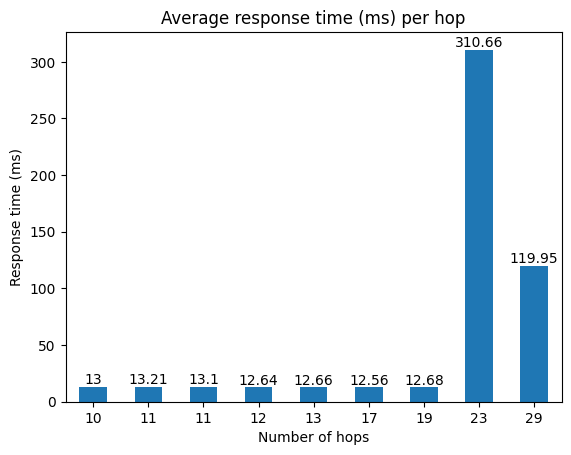
\includegraphics[width=0.49\textwidth]{time_num_hops.png}
                \caption{\small Latency vs hops}
                \label{fig:time_hops}
        \end{figure}
\noindent



\subsection{Quality of Measurements}
All the results suffer by several limitations that can be accepted since the goal of this project is just to explore the DNS structure and the tools that can be exploit to assess its performance. 
First of all the experiments have been conducted on a Ubuntu operating system which can have a different implementation of the stub resolver 
respect to other operating systems, leading to different results. Second, a single vantage point has been used and this provide a very restricted view of the DNS performance. Third, 
the results are strongly affected by the network traffic. Repeating the experiment on a vacation day, the average latency using UDP for 8.8.8.8 in the same experiment setup
as in point 6, changes from 0.035 to 0.23 seconds.


\subsection{Conclusions}
All the public DNS server showed good and stable performance. The one provided by Google is the fastest overall but the gaps are very tight. The query resolution time is strongly affected
by the protocol used. The encrypted protocols are slower than the unencrypted ones with DoH slower than DoT. The usage of TCP protocol and the DNSSEC option lead to 
an increasing in the latency as well. The distance between the client and the DNS server used is another important factor when it comes to the latency, the
more far the server the higher the time for query resolution. Finally, the type of query can influence the latency as well, but the differences are not so significant.\\


\section{General Conclusions}
These two projects introduced me to a totally new domain, that of the digital infrastructures. They made me conscious about the complexity of this field and the several variables impacting it.
It requires a significant amount of effort to get enough domain-specific knowledge to generate meaningful results and draw conclusive insights. These aspects make the realm of digital infrastructures 
a very catching one to my eyes.


%Insert couple of sentences that highlight the lessons you have learnt (if any) from these lab activities.

        
\end{multicols}
%\section{References}
%Insert bibliographical references (if any) you might have used for your lab activities.
\end{document}